\documentclass{protokoll}
\newcommand{\assistent}{N. Spethmann}
\newcommand{\versuch}{High Resolution Laser Spectroscopy}
\newcommand{\nummer}{A246}

\newcommand{\vr}[2]{\ensuremath{\left(\begin{array}{c}#1\\#2\end{array}\right)}}

\begin{document}

\section{Einleitung}
Dieser Versuch soll einen Einblick in die Anwendung von Lasern f�r hochaufl�sende atomare Spektroskopie geben. Hierzu werden zun�chst die Leistung des Diodenlasers in Abh�ngigkeit vom Injektionsstrom und Finesse des zur Verf�gung stehenden \textsc{Fabry-Perot}-Interferometers bestimmt. Zur Ausmessung ausgew�hlter Linien von Rubidium wird anschlie�end der Aufbau erweitert, um lineare Spektroskopie sowie S�ttigungsspektroskopie durchf�hren zu k�nnen.

\section{Theoretische Grundlagen}
\subsection{Diodenlaser}

\subsection{Fabry-Perot-Interferometer}
\subsection{Lineare Spektroskopie}
\subsection{S�ttigungsspektroskopie}
\subsection{Eigenschaften von Rubidium}


\section{Versuchsdurchf�hrung und Auswertung}
\subsection{Charakteristik des Diodenlasers}\label{subsec:Ana_DiodeLaser}
Zuerst sollen einige Kenngr��en des Diodenlasers, n�mlich Schwellenstrom $I_\mathrm{thr}$, differentieller Wirkungsgrad $\partial P_\mathrm{out} / \partial I$ und Quanteneffizienz $\eta$, bestimmt werden. Dazu verwenden wir den in Abbildung \ref{fig:Aufbau_Laserdiode} gezeigten Aufbau und messen die Ausgangsleistung der Diode in Abh�ngigkeit vom Eingangsstrom. 
\begin{figure}[H]
	\centering
		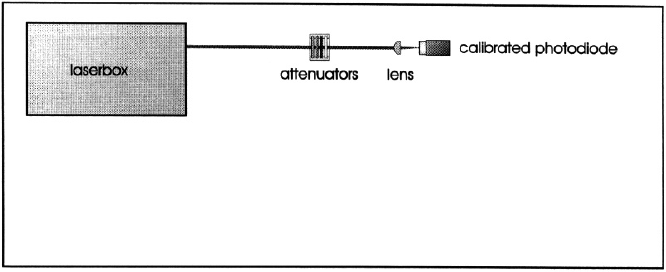
\includegraphics[width=0.8\textwidth]{graphics/Aufbau_Laserdiode}
	\caption{Aufbau zur Bestimmung der Kenngr��en der Laserdiode}
	\label{fig:Aufbau_Laserdiode}
\end{figure}
Wir erhalten die in Tabelle \ref{tab:Laserdiode} im Anhang aufgef�hrten und in Abbildung \ref{fig:Laserdiode_Plot} graphisch dargestellten Daten. 
\begin{figure}[H]
	\centering
		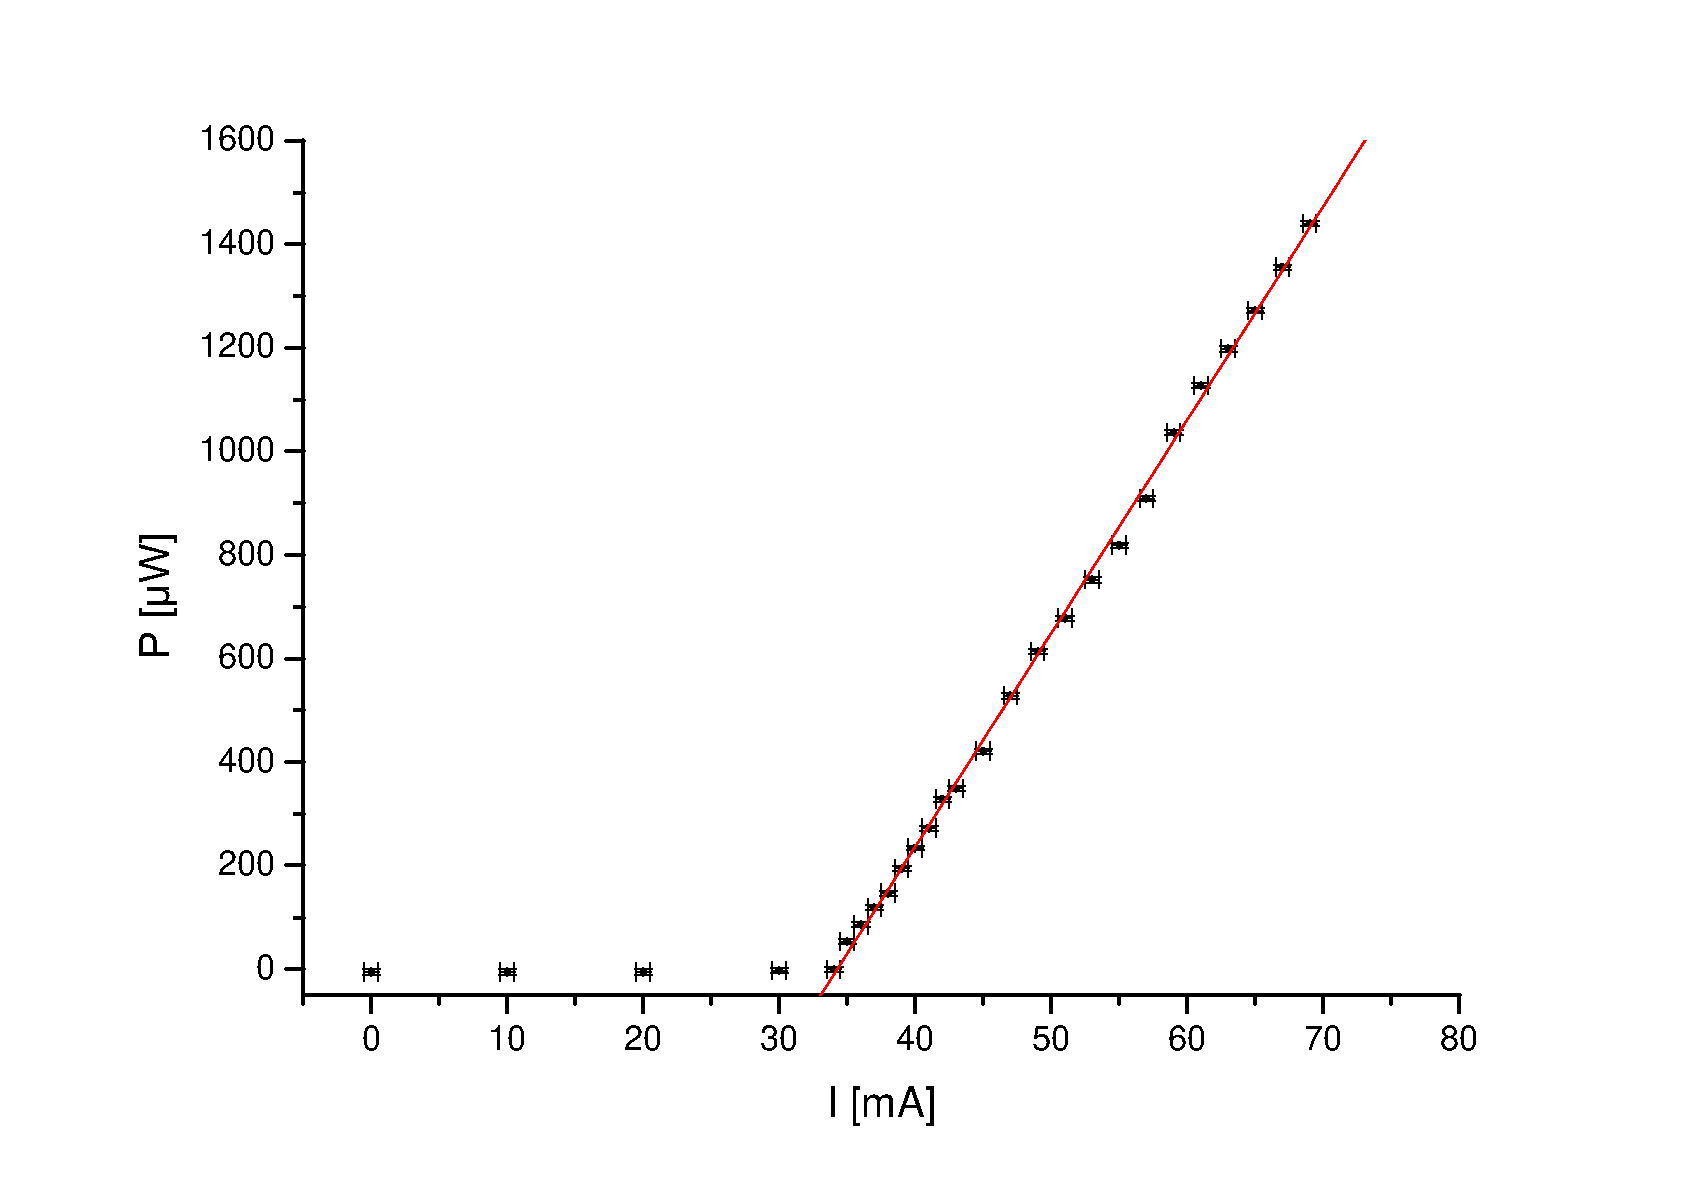
\includegraphics[width=1.0\textwidth]{graphics/Laserdiode_Plot}
	\caption{Plot der Messergebnisse zur Bestimmung der Kenngr��en der Laserdiode mit Fit an den linearen Bereich}
	\label{fig:Laserdiode_Plot}
\end{figure}
Man erkennt f�r kleine Str�me einen langsamen Anstieg der Leistung mit dem Eingangsstrom, der ab dem so genannten Schwellenstrom deutlich st�rker wird. Ein Geradenfit an diesen als linear approximierten Anstieg liefert:
\begin{align}
P = m\cdotp I + b=\unit[(41.218 \pm 0.009)]{\frac{\mu W}{mA}} \,\cdotp\, I - \unit[(1412.3 \pm 0.4)]{\mu W}
\end{align}
Der differentielle Wirkungsgrad ist identisch zur Steigung der Geraden, der Schwellenstrom berechnet sich nach $I_\mathrm{thr}=-\frac{b}{m}$ und f�r die Quanteneffizienz gilt:
\begin{align}
\eta = \frac{N_\gamma}{N_\mathrm{e}} = \frac{Pe}{I h \nu} = \frac{\partial P}{\partial I} \frac{e\lambda}{hc} \ldotp
\end{align}
Damit ergeben sich die in Tabelle \ref{tab:Laserdiode_Kenngroessen} zusammengefassten Kenngr��en der Diode.
\begin{table}[H]
  \centering
\resizebox{0.5\textwidth}{!}{
  \begin{tabular}{lc}
    \toprule
      & bestimmter Wert\\
    \midrule[0.75pt]
Schwellenstrom & $\unit[(34.26 \pm 0.01)]{mA}$\\
differentieller Wirkungsgrad & $\unit[(41.218 \pm 0,009)]{\frac{\mu W}{mA}}$\\
Quanteneffizienz & $26.422 \pm 0.006$\\
    \bottomrule
  \end{tabular}
}
 \caption{Zusammenfassung der Kenngr��en der Laserdiode}
  \label{tab:Laserdiode_Kenngroessen}
\end{table}



\subsection{Fabry-Perot Interferometer}\label{subsec:Ana_FabryPerot}
Zur Untersuchung des \textsc{Fabry-Perot}-Interferometers (FPI) verwenden wir den in Abbildung \ref{fig:Aufbau_FPI} dargestellten Versuchsaufbau.
\begin{figure}[H]
	\centering
		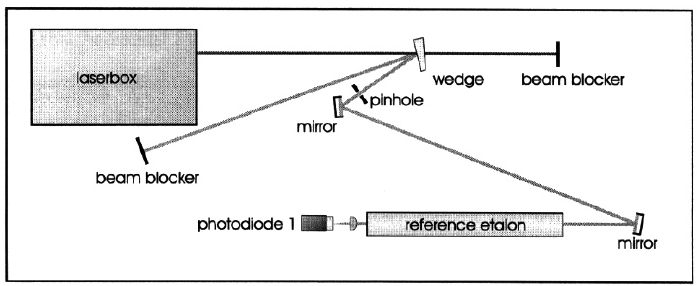
\includegraphics[width=0.8\textwidth]{graphics/Aufbau_FPI}
	\caption{Aufbau zur Untersuchung des Fabry-Perot Interferometers}
	\label{fig:Aufbau_FPI}
\end{figure}
Mittels eines Glaskeils wird der Laserstrahl in drei Teilstrahlen aufgespalten, von denen zwei mithilfe geschw�rzter Platten blockiert werden. Der verbleidende Strahl wird nach Durchgang durch eine Lochblende, die R�ckreflexionen in den Laser vermeiden soll, mithilfe zweier Spiegel durch das Interferometer gelenkt. Der vom Interferometer transmittierte Strahl wird mit einer Linse auf eine Photodiode fokussiert, deren Ausgangssignal wir auf einem Oszilloskop betrachten. Mittels des in der Laserbox enthaltenen \textsc{Littrow}-Gitters stimmen wir den Laser periodisch durch Anlegen einer S�gezahn-Spannung durch. Dabei benutzen wir den Trigger-Ausgang des Funktionsgenerators zum Triggern des Oszilloskops. Nach Optimierung der Justage durch Maximierung der Spannungsamplitude der Photodiode erhalten wir das in Abbildung \ref{fig:FPI_Plot} ausschnittsweise gezeigte Oszillogramm.
\begin{figure}[H]
	\centering
		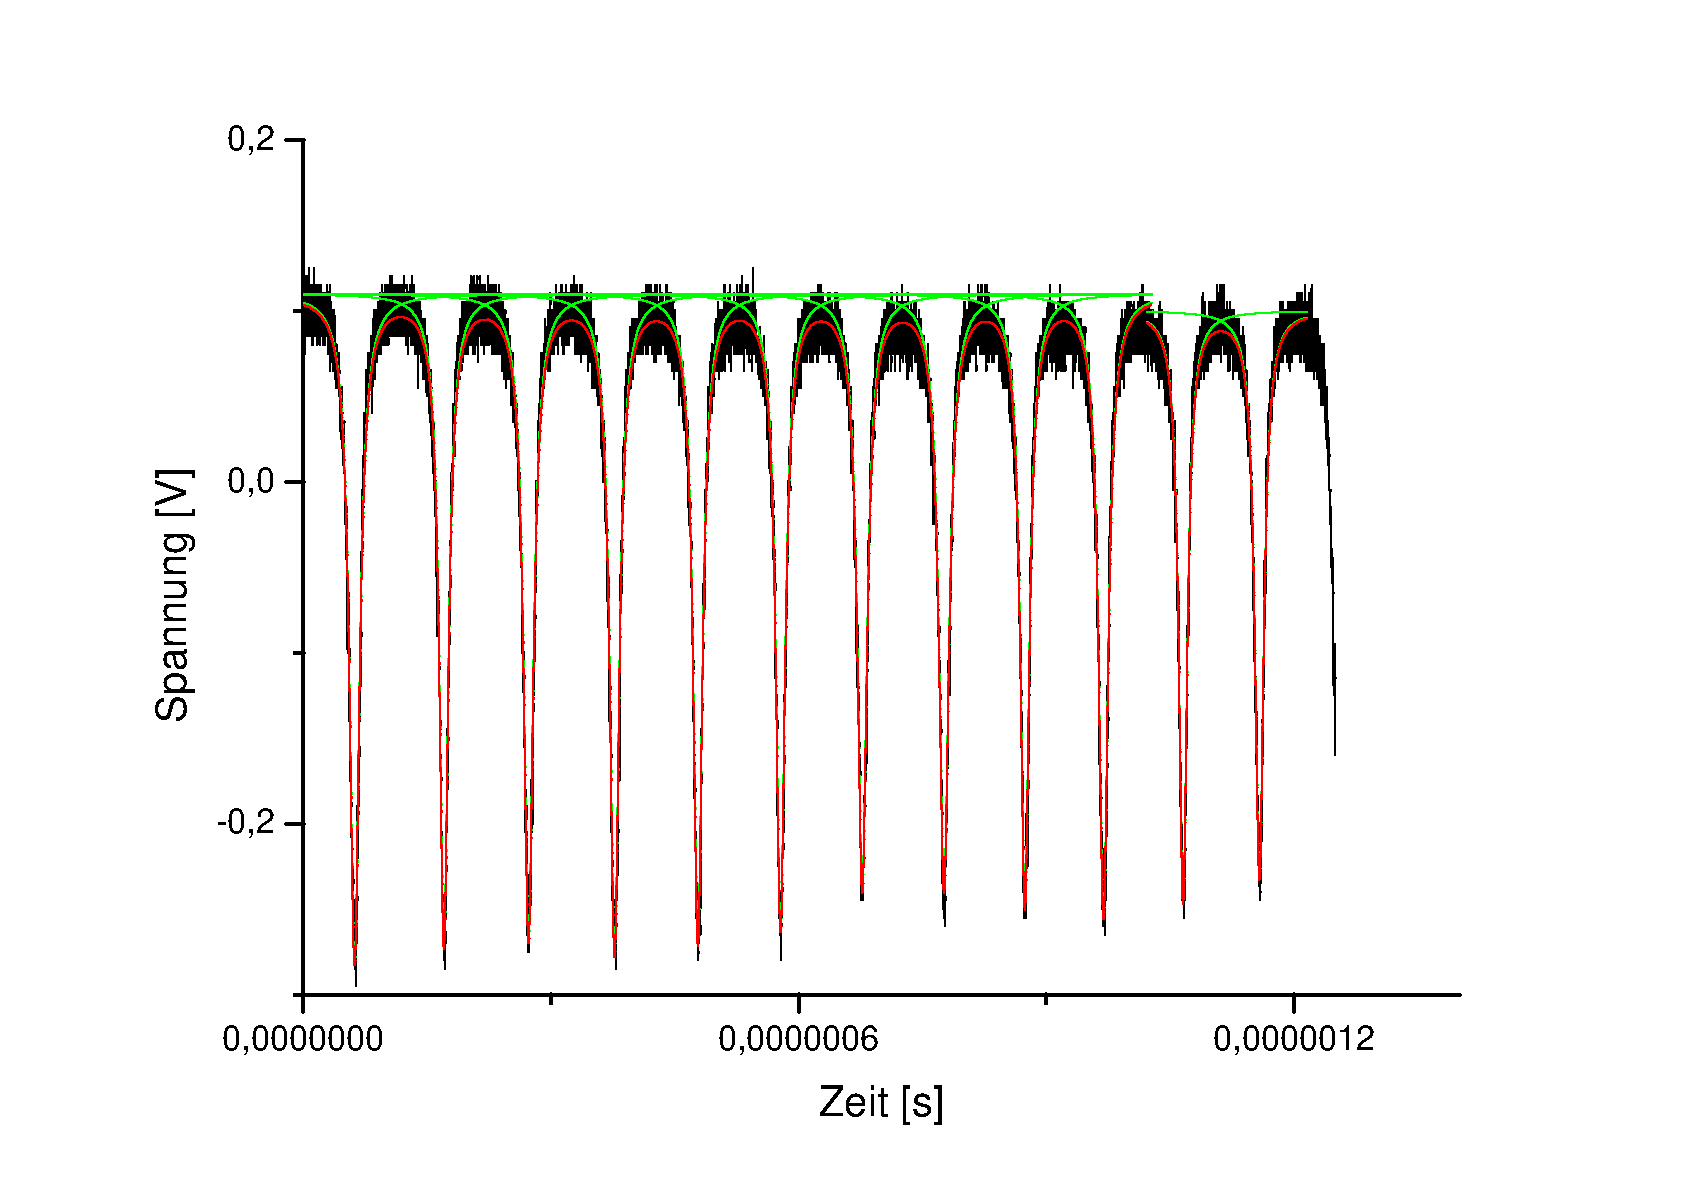
\includegraphics[width=1.0\textwidth]{graphics/FPI_Plot}
	\caption{Ausschnitt aus dem an der Photodiode gemessenen Oszillogramm mit \textsc{Lorentz}-Fits}
	\label{fig:FPI_Plot}
\end{figure}
Zur Bestimmung der Finesse des \textsc{Fabry-Perot}-Interferometers passen wir \textsc{Lorentz}-Kurven an die Peaks des Oszillogramms an. Aus den Fit-Parametern ergibt sich die Finesse gem��:
\begin{align}
\mathcal{F} = \frac{\delta \nu}{\Delta \nu} \ldotp
\end{align}
Wir sch�tzen auf die Spannungswerte einen Fehler von $\unit[0.01]{V}$, auf die Zeitablenkung jeweils einen Fehler von $\unit[0.0005]{\mu s}$. Aus den Fits erhalten wir die in Tabelle \ref{tab:FPI_Data} im Anhang zusammengefassten Werte. Dabei berechnen wir die Finesse f�r jeden Peak einzeln. Wobei sich der Fehler jeweils aus \textsc{Gau�}scher Fehlerfortpflanzung ergibt.

Der fehlergewichtete Mittelwert ergibt sich zu:
\begin{align}
\mathcal{F} = (7.282 \pm 0.002) \ldotp
\end{align}
Nach Abschnitt XXX ist die Finesse gegeben durch:
\begin{align}
\mathcal{F} = \frac{\pi \sqrt{R}}{1-R}
\end{align}
und die Reflektivit�t der Spiegel des Interferometers ist (nach~\cite{skript}) $R=0.9$. Damit erh�lt man f�r die Finesse den theoretischen Wert von
\begin{align}
\mathcal{F}_\mathrm{th} = 29.804 \ldotp
\end{align}
Die von uns gemessene Finesse betr�gt also nur ca. $1/4$ des theoretischen Werts. Dies liegt wahrscheinlich an einer zu ungenauen Justage, k�nnte aber auch durch eine Reflektivit�tsminderung der Spiegel durch Alterungsprozesse bedingt sein.

Nun soll anhand des bekannten Frequenzabstands der Peaks des Interferometers eine Eichkurve f�r die Zeitachse bestimmt werden. Dazu fitten wir \textsc{Lorentz}-Kurven an eine m�glichst gro�e Zahl von Peaks im Spektrum des FPI und tragen die Peakpositionen gegen ihre relative Frequenz auf. Der Nullpunkt der Frequenzskala wird dabei willk�rlich gew�hlt. Das Ergebnis ist in Abbildung \ref{fig:FPI_GaugeFit} zu sehen.
\begin{figure}[H]
	\centering
		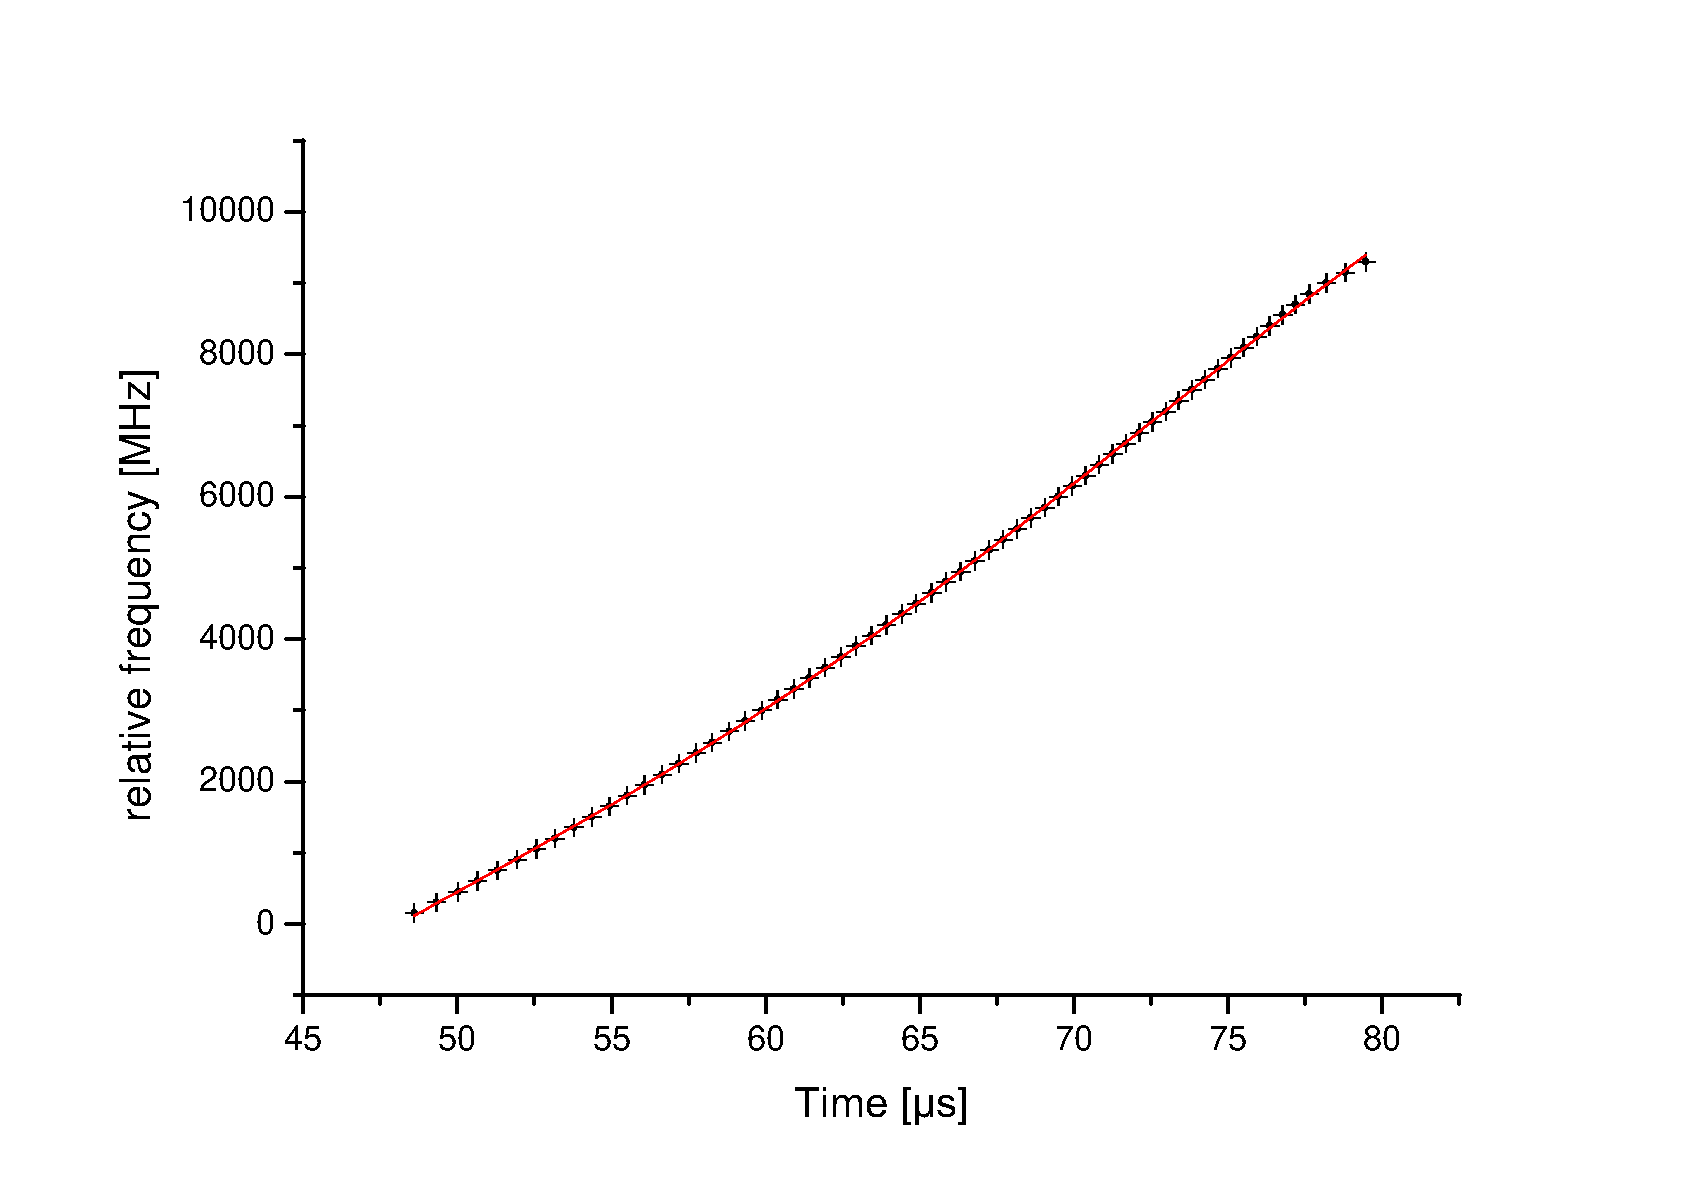
\includegraphics[width=1.0\textwidth]{graphics/FPI_GaugeFit}
	\caption{Positionen der Peaks des FPI gegen die relative Frequenz mit Fit}
	\label{fig:FPI_GaugeFit}
\end{figure}
Da die Kurve leicht nicht-linear verl�uft, passen wir ein Polynom zweiten Grades an die Daten an. Das Ergebnis des Fits lautet:
\begin{align}
    f(t) &= a + b\,\cdotp\, t + c\, \cdotp\, t^2 \hspace{2cm}\mathrm{mit:}\\
\notag a &= \unit[(-5739.032 \pm 0.002)]{MHz} \\
\notag b &= (6.73776 \pm 0.00005)\\
\notag c &=\unit[(2.3302300 \pm 0.0000004)]{\frac{1}{\mu s}}
\end{align}


\section{Zusammenfassung}

\begin{appendix}
\section{Tabellen}
\begin{table}[H]
  \centering
\resizebox{0.5\textwidth}{!}{
  \begin{tabular}{cc}
    \toprule
     $I$ [mA] $\pm$ 0,5 mA & $P$ [$\mu$W] $\pm$ 5 $\mu$W\\
    \midrule[0.75pt]
$0$	&$-6$\\
$10$	&$-6$\\
$20$	&$-6$\\
$30$	&$-3$\\
$34$	&$-1$\\
$35$	&$53$\\
$36$	&$85$\\
$37$	&$119$\\
$38$	&$147$\\
$39$	&$194$\\
$40$	&$234$\\
$41$	&$272$\\
$42$	&$328$\\
$43$	&$349$\\
$45$	&$421$\\
$47$	&$528$\\
$49$	&$613$\\
$51$	&$678$\\
$53$	&$752$\\
$55$	&$819$\\
$57$	&$909$\\
$59$	&$1036$\\
$61$	&$1127$\\
$63$	&$1198$\\
$65$	&$1272$\\
$67$	&$1356$\\
$69$	&$1440$\\
    \bottomrule
  \end{tabular}
}
  \caption{Messergebnisse bei Messung der Diodenausgangsleistung in Abh�ngigkeit vom Eingangsstrom}
  \label{tab:Laserdiode}
\end{table}

\begin{table}[H]
  \centering
\resizebox{1.0\textwidth}{!}{
  \begin{tabular}{l|cc|cc}
    \toprule
      Peak & $\nu_0$ [$\unit[10^{-8}]{s}$] & $\Delta \nu$ [$\unit[10^{-8}]{s}$] & $\delta \nu$ [$\unit[10^{-8}]{s}$] & $\mathcal{F}$\\
    \midrule[0.75pt]
$1$ & $6.206 \pm 0.003$ & $1.441 \pm 0.009$ & $10.819  \pm 0.004$ & $7.509 \pm 0.045$\\
$2$ & $17.025 \pm 0.003$ & $1.299 \pm 0.008$ & $10.252 \pm 0.004$ & $7.893 \pm 0.051$\\
$3$ & $27.277 \pm 0.003$ & $1.404 \pm 0.009$ & $10.420 \pm 0.004$ & $7.421 \pm 0.047$\\
$4$ & $37.697 \pm 0.003$ & $1.375 \pm 0.009$ & $10.088 \pm 0.004$ & $7.334 \pm 0.046$\\
$5$ & $47.785 \pm 0.003$ & $1.343 \pm 0.009$ & $10.011 \pm 0.004$ & $7.455 \pm 0.048$\\
$6$ & $57.795 \pm 0.003$ & $1.338 \pm 0.009$ & $9.900  \pm 0.004$ & $7.397 \pm 0.049$\\
$7$ & $67.696 \pm 0.003$ & $1.415 \pm 0.010$ & $9.903  \pm 0.005$ & $7.000 \pm 0.048$\\
$8$ & $77.599 \pm 0.003$ & $1.473 \pm 0.010$ & $9.791  \pm 0.005$ & $6.646 \pm 0.045$\\
$9$ & $87.389 \pm 0.003$ & $1.322 \pm 0.009$ & $9.518  \pm 0.004$ & $7.200 \pm 0.049$\\
$10$ & $96.907 \pm 0.003$ & $1.391 \pm 0.009$ & $9.639 \pm 0.004$ & $6.931 \pm 0.046$\\
$11$ & $106.546 \pm 0.003$ & $1.213 \pm 0.010$ & $9.244\pm 0.004$ & $7.619 \pm 0.062$\\
$12$ & $115.790 \pm 0.003$ & $1.277 \pm 0.011$ &  & \\
    \bottomrule
  \end{tabular}
}
\caption{Fit-Ergebnisse der Bestimmung der Finesse des Interferometers}
  \label{tab:FPI_Data}
\end{table}

\Literatur{quellen}

\end{appendix}
\end{document}


